%%% -*- coding: utf-8 -*-
\newpage

\chapter{Theory and technical background}
\label{chap:theory}

This Chapter aims to set a basic understanding on the concepts underlying the techniques used in this Dissertation.

\section{Artificial Neural Networks}\label{sec:NNs}

Artificial Neural Networks (ANNs) are machine learning models inspired by the Biologic Neuron. The Perceptron~\cite{rosenbaltt1957perceptron} is one of the main precursors of modern ANNs. The Perceptron is a mathematical model of the Neuron, it is capable of binary classification. It draws its differentiation power from adjusting a linear function with its weights. It can differentiate any linearly separable problem, that is, any problem in which a hyperplane (a plane in multiple dimensions) can separate the two classes of the data.

A Perceptron receives $m$ inputs, denoted $X$, it holds $m$ weights $W$, one weight for each input, and a $bias$. During training, the weights $W$ and the $bias$ are adjusted in order to optimize hyperplane separation.

\begin{figure*}[!ht]
    \centering
    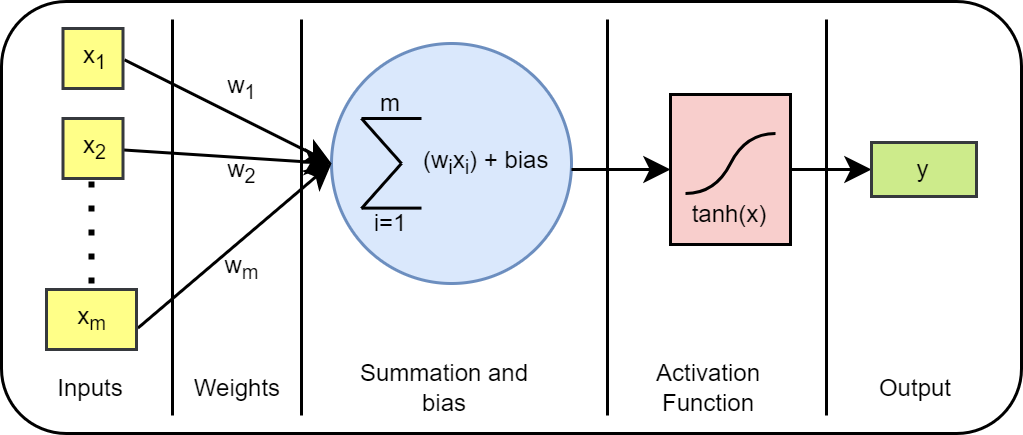
\includegraphics[width=0.95\textwidth]{img/Perceptron.drawio.png}
    \caption{The Perceptron and its components, the input layer, the weights, the weighted sum and bias, the activation function and the output layer.}
    \label{fig:perceptron}
\end{figure*}

To obtain the output of a Perceptron (a prediction), its weights are multiplied by the inputs, then the sum of these multiplications are summed and then a bias is added this result. This weighted sum of the input features can be calculated through Equation \ref{eq:perceptron}. 
%https://www.sciencedirect.com/topics/computer-science/multilayer-perceptron
\begin{equation}\label{eq:perceptron}
\displaystyle\sum_{i=1} ^{m} (x_i w_i)+bias
\end{equation}
Where $m$ is the number of inputs, $x_i$ and $w_i$ are the inputs and weights and $i$ is the number of the input. Finally, the weighted sum of the input features (and bias) are input through an activation function, which in the original perceptron is a \textit{Step function}, but in Figure \ref{fig:perceptron}, which shows a diagram of the Perceptron structure, is a \textit{Hyperbolic tangent} function. The result of the activation function is the output of the Perceptron.

The learning process of the Perceptron is adjusting the weights and the bias so that the hyperplane can separate the training data up to a set metric.

%While the Perceptron can only solve Linearly separable problems, the Multi Layer Perceptron (MLP) can solve non-Linear problems. 
By stacking layers of multiple Perceptrons, one can approximate any continuous function, rather than only linear functions, thus being able to solve both linear and non-linear problems. MLPs are also known as Fully Connected (FC) neurals networks when combined with other modern neural networks.
The general structure of a Multi Layer Perceptron (MLP), as shown in Figure \ref{fig:mlp-structure} consists on a input layer, one or more hidden layers, and a output layer.

\begin{figure*}[!ht]
    \centering
    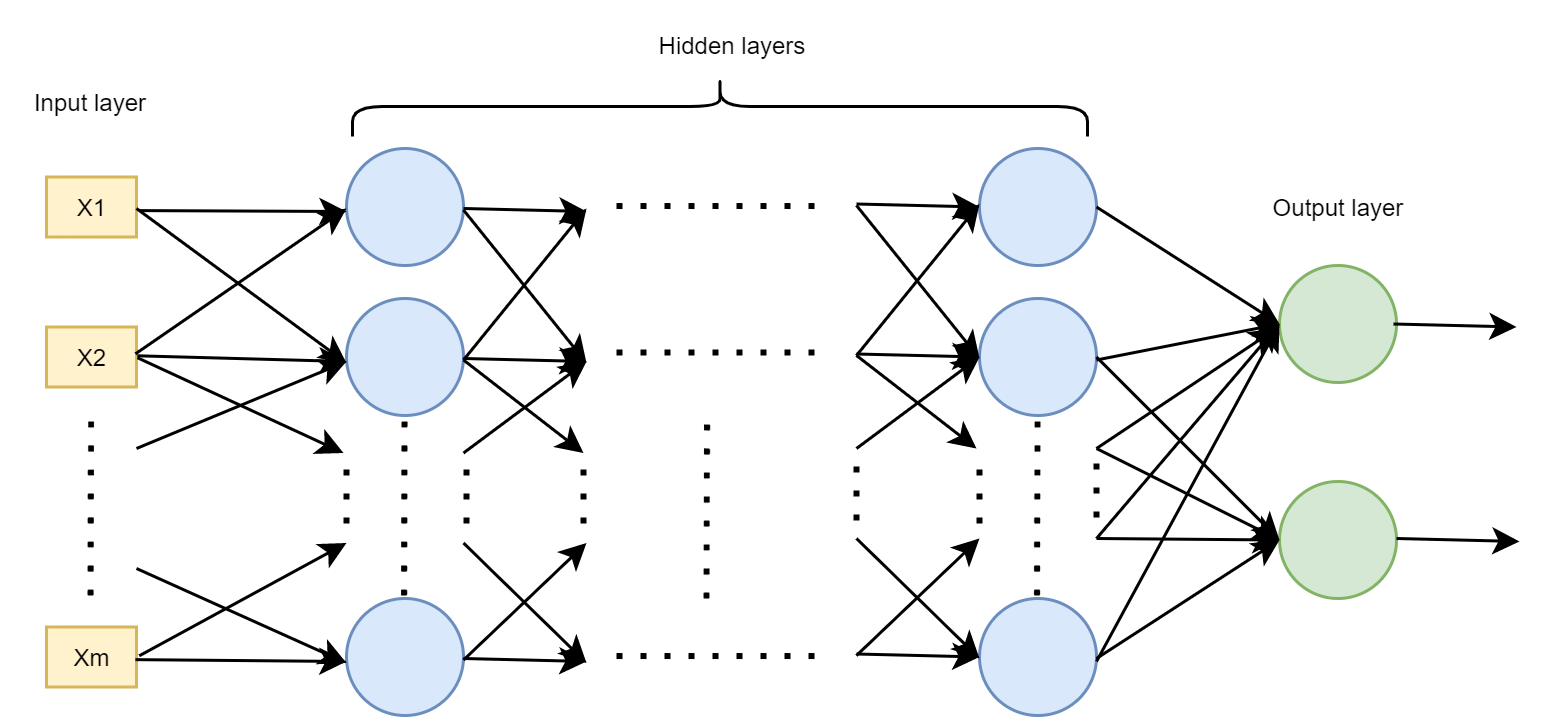
\includegraphics[width=0.95\textwidth]{img/MLP.drawio.png}
    \caption{The Multi Layer Perceptron}
    \label{fig:mlp-structure}
\end{figure*}

The training procedure for the MLP is called \textit{Backpropagation}. It is a process in which the loss value is calculated to measure the error rate of a output. The loss value is used to adjust the weights of the neural network in the reverse sequence of the prediction process. Gurney et. al.\cite{gurney2018introduction} further details the Perceptron and the Multi Layer Perceptron and how the learning on each of them occurs.

When training MLPs, some problems may arise. Overfitting and Underfitting, are, respectively, learning to match the exact pattern of the training data, and not approximating (or learning) the desired pattern enough, in both cases, the network fails to generalize to data outside of the training set. For Overfitting, there are many techniques that mitigate this problem, such as dropout (when some neurons are randomly deactivated when training), and cross validation (split training set in chunks and training with random chunks). Underfitting, on the flip side, may mean that the complexity of the model is too small for the train set or that the training data is insufficient. 
%or learning rate (the size of Backpropagation adjustments)

\section{Convolutional Neural Networks}\label{sec:CNN}


The concept of Neural Networks can also be applied on to computer vision, by combining the concept of convolutions and neural networks, Kunihiko Fukushima created the precursor of modern Convolutional Neural Networks (CNNs), the "neocognitron"\cite{neocognitron1980} in 1980.

To understand CNNs, one must first understand the convolution operation, used in many image processing techniques.
%https://vincmazet.github.io/bip/filtering/convolution.html
\begin{figure*}[!ht]
    \centering
    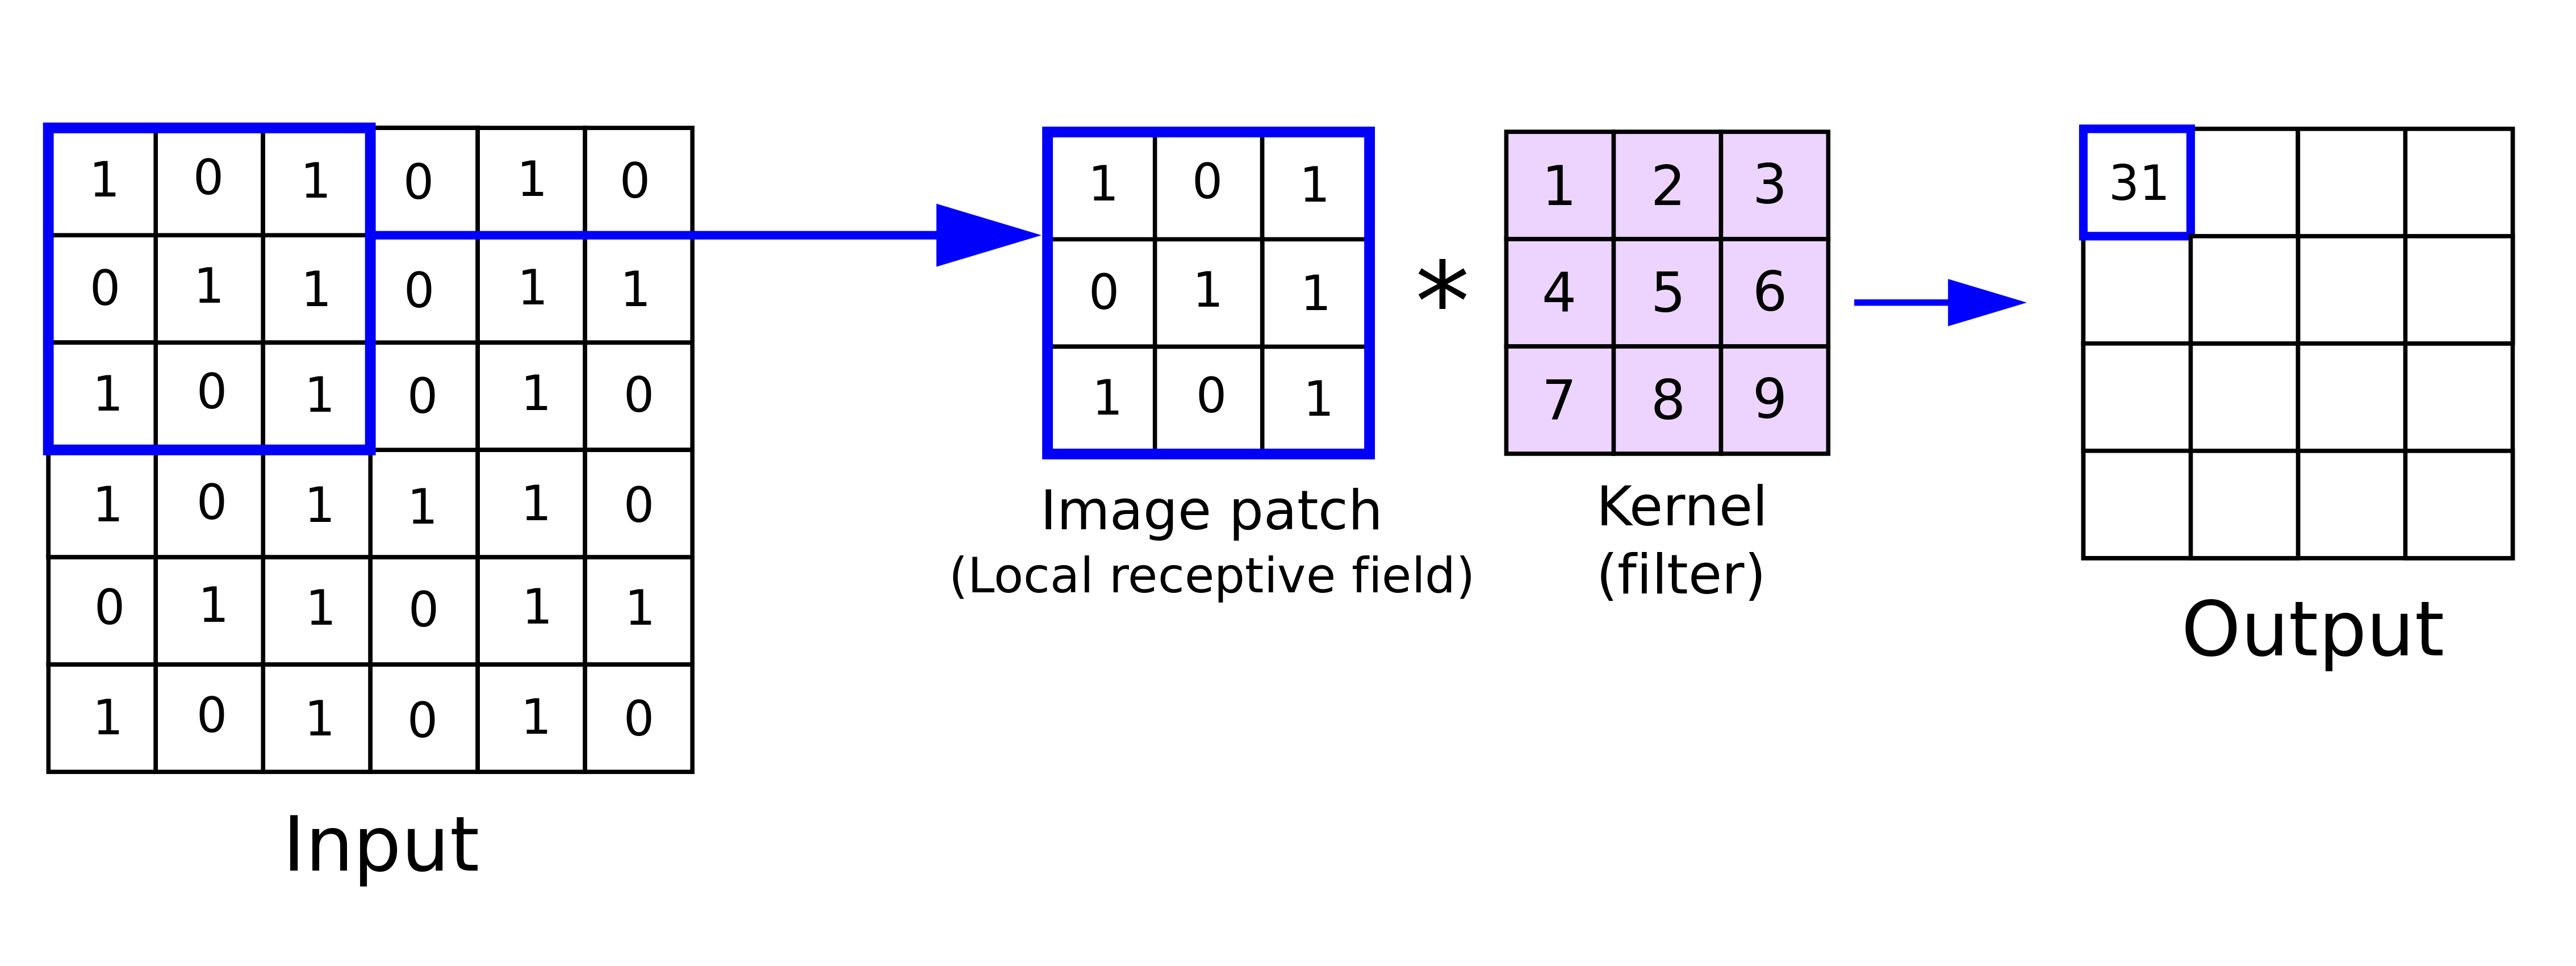
\includegraphics[width=0.95\textwidth]{img/convolution.png}
    \caption[The Convolution Operation]{The Convolution operation, this is the main operation behind Convolutional Neural Networks. Image author: Anh H. Reynolds\footnotemark}
    \label{fig:convolution}
\end{figure*}
%https://anhreynolds.com/blogs/cnn.html

Convolutions consist on applying a filter (or mask), a matrix of values, to a image. As exemplified in Figure \ref{fig:convolution}\footnotetext{\url{https://anhreynolds.com/blogs/cnn.html}}. The operations consists on multiplying each value on the mask for the equivalent pixel (on the current image patch) in the image, then sum all results of these multiplications, this will be the new pixel value of the resulting image/feature map.

%\pva{formula aqui?}

In CNNs, each value of the filter is learned, as if the wheights to be learned in the neural networks are now the values of the convolutional mask.
Each convolution layer has its learned weights for their filters, therefore each convolution layer will process the inputs even further, each layer passing its output to the next.


CNNs also use an operation called Pooling in order to reduce the size of the of the input of a layer (downsample), and consequently speed up computation, by "distilling" the features they become more robust to noise.

The two most common methods of pooling are average and max pooling. Max pooling takes the max value of each neighboring neurons/inputs while average pooling is the average value of each neighboring neurons/inputs. As represented in Figure \ref{fig:avgmax-pooling}.

There are also two different ways to perform Pooling operations. Local pooling reduces the output of the previous neurons/inputs per channel.
Global pooling combines values of previous neurons/inputs across dimensions, or channels, in the feature map. 

%https://androidkt.com/explain-pooling-layers-max-pooling-average-pooling-global-average-pooling-and-global-max-pooling/
\begin{figure*}[!ht]
    \centering
    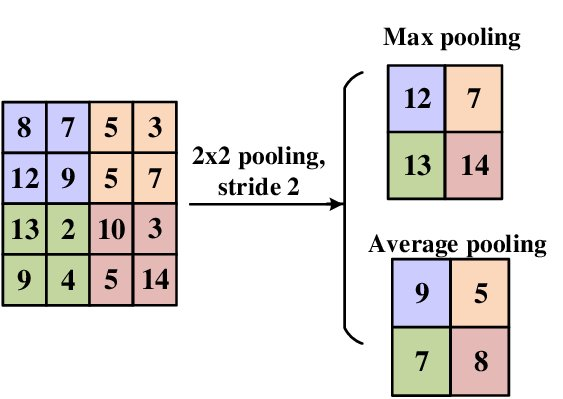
\includegraphics[width=0.55\textwidth]{img/pooling.jpg}
    \caption{Local Max and Average Pooling representation. Image authors are Yingge et. al.\cite{yingge2020pooling}}
    \label{fig:avgmax-pooling}
\end{figure*}

In the first stage of a traditional image classification CNN is comprised of convolutional and pooling layers, extracting and disitlling characthistics as the layers get deeper into the model, this is called the feature extraction stage. Then, the features are input to the classification stage, which is usually a fully connected layer of neurons (a Multilayer Perceptron). The classification stage outputs 
%the activations or probabilities for each class, which then are used to decide 
the predicted class. This generic image classification CNN is shown in Figure \ref{fig:generic-cnn}.
%in the 1980s by Yann LeCun, a postdoctoral computer science researcher.
\begin{figure*}[!ht]
    \centering
    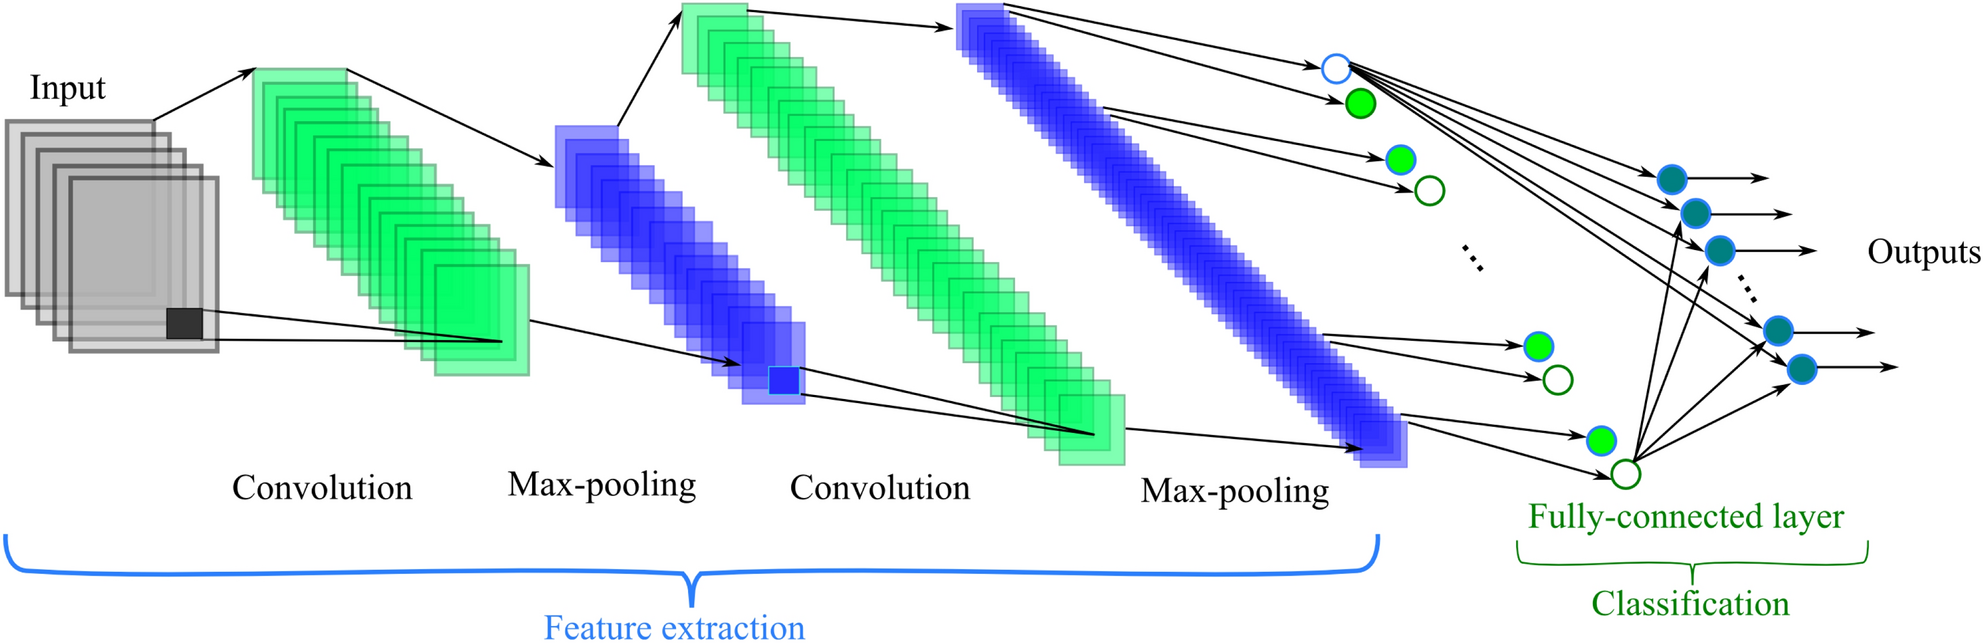
\includegraphics[width=0.95\textwidth]{img/generic-convnet.png}
    \caption{A generic image classification CNN architecture, representing the feature extraction stage and the classification stage. Note that as the inputs progress through the CNN the width and height of the inputs become smaller, but the number of feature channels/dimensions increases. Image authors are Khozeimeh et. al.\cite{khozeimeh2021cnnimage}}
    \label{fig:generic-cnn}
\end{figure*}

As convolutional layers get deeper, the level of abstraction also gets higher, as an example, in a generic image classification CNN, the last layers the features may represent more abstract concepts, such as the presence of objects and complex shapes such as cars. These abstractions depend on what images the CNN was trained and what is it supposed to classify. 

Once a CNN is trained with success, it should have learned representations as features that allow it to differentiate between classes. By training a new classifier on the already existent learned concepts (features) in the last convolutional layers, one can modify this generic CNN to classify between dogs and cats or types of car. One could also use the same trained generic CNN and continue training it on a different task, using the already learned concepts as a head start, the CNN would also learn more specific concepts to this task as the training continues. This is called transfer learning. 

%2009
One of the most popular datasets and challenges for CNNs is the The ImageNet Large Scale Visual Recognition Challenge (ILSVRC)\footnote{\url{http://www.image-net.org/}}\cite{deng2009imagenet}, in 2012 it hosted the work that ushered a boom in CNN research and development when AlexNet achieved a top-5 error of 15.3\% in the ILSVRC, more than 10.8 percentage points lower than that of the second place. The ImageNet dataset has more than 100.000 "synonym sets" which are sets of words or phrases that represent the image. The dataset holds multiple challenges for tasks such as Image classification, Single-object localization and Object detection, each of the subsets for these tasks have 1000 classes (or objects).

A CNN trained on the ImageNet dataset, can learn a wide variety of abstractions, from cars to dogs, because of the wide scope of their image classification task. This makes CNNs pre-trained in the ImageNet dataset specially performant as transfer learning models~\cite{huh2016makes}.

With the success of CNNs, researchers started modifying and applying these models on other domains, such as audio, time series and natural language processing.

The equivalent of the ImageNet dataset for the audio classification is the Audioset\footnote{\url{https://research.google.com/audioset/}}~\cite{gemmeke2017audioset}. It is an ontology of 632 audio classes and 2,084,320 human-labeled 10-second sound clips collected from YouTube videos. Its classes range from human and animal sounds, musical instruments and genres, and common everyday environmental sounds.

With the advent of deeper CNNs, one problem also surfaced: The vanishing gradient problem, it occurs when the error propagation makes the training diverge, the values of weights become too small. To avoid this problem, there are multiple techniques, such as the Rectified Linear Unit (ReLU) activation function~\cite{krizhevsky2012relu}, and lower the learning rate, thus taking smaller steps when adjusting the weights.

\section{The VGG Convolutional Neural Network}\label{sec:VGGish}

The VGG Convolutional Neural Network~\cite{simonyan2014VGG} was designed for the ImageNet Challenge in 2014, where it won the first and second place in localization and classification tasks. It's input is a 224$\times$224 RGB image. The main contribution of this network is that is showed that even with a very small receptive field (3$\times$3, which is the smallest size to capture the notion of left/right, up/down and center, by increasing the depth of a network, it could still outperform all other CNN based methods at the time.

This architecture has 6 configurations with different depths that are connected to two Fully Connected (FC) layers, two of 4096 channels and a final one with a 1000 channels (The Image Net challenge had a 1000 classes), followed by a soft-max layer that outputs the predicted class.
The configuration of the fully connected layers is the same in all configurations. All hidden layers used rectification (ReLU)~\cite{krizhevsky2012relu} non-linearity. Figure \ref{fig:vgg16} shows the most popular variation, the VGG-16 (Configuration D) and its layers, as described above.

\begin{figure*}[!ht]
    \centering
    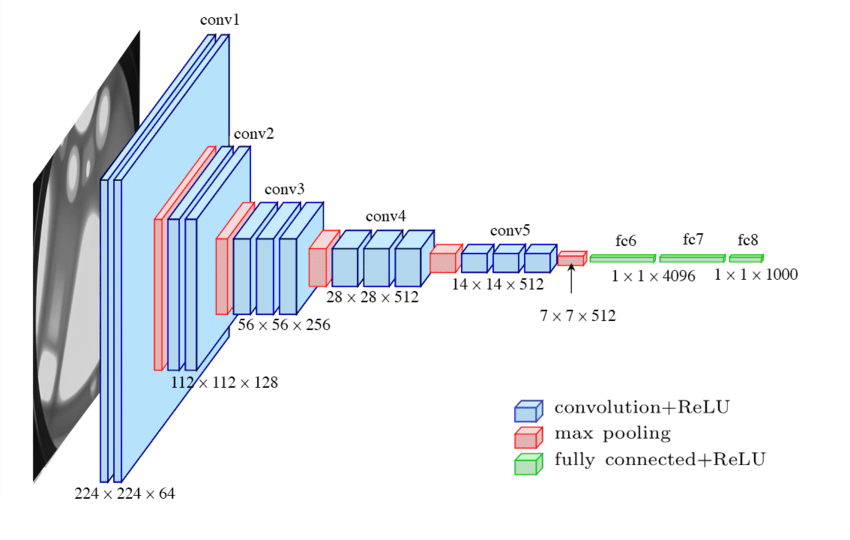
\includegraphics[width=0.95\textwidth]{img/vgg16.png}
    \caption{VGG-16 architecture, image authors are Ferguson et. al.\cite{ferguson2017vggimage}.}
    \label{fig:vgg16}
\end{figure*}

\section{VGGish}\label{sec:VGGish}
The VGGish is a variation of the VGG-11 (Configuration A), created by the authors of the YouTube8m dataset ~\cite{abu2016youtube}, with some modifications to perform audio (spectogram) classification and embeddings generation).

Specifically, the input size was modified to 96$\times$64 for log mel spectogram audio inputs. The last group of convolution and maxpool layers were removed. In order to created a compact embedding layer, the 1000 channels wide FC layer at the end was changed to a 128-wide FC layer. This final layer does not have an non-linear activation.

\section{The Inception Convolutional Neural Network}\label{sec:Inception}

The Inception Convolutional Neural Network or GoogLeNet, ~\cite{szegedy2015Inception} was designed for the ImageNet Large-Scale Visual Recognition Challenge in 2014, it features many techniques in order to increase efficiency of deep CNNS.

In order to achieve this increased efficiency, the authors created a module to capture as much information as possible, both in local and global context, by using multiple kernel sizes in the same convolutional layer. To optimize for computational cost and speed, the creators also avoided naively stacking layers, for it is computationally expensive.

The solution proposed by the authors of the inception CNN is to use compute multiple filters in the same level, with varying convolutional filter sizes.

The ``Naive'' inception module, as shown in Figure \ref{fig:naive-inception} consists on a convolutional layer using 3 different filter sizes, 1$\times$1, 3$\times$3 and 5$\times$5. Along with a max pooling operation. The outputs are then concatenated by the end of the inception module.

\begin{figure*}[!ht]
    \centering
    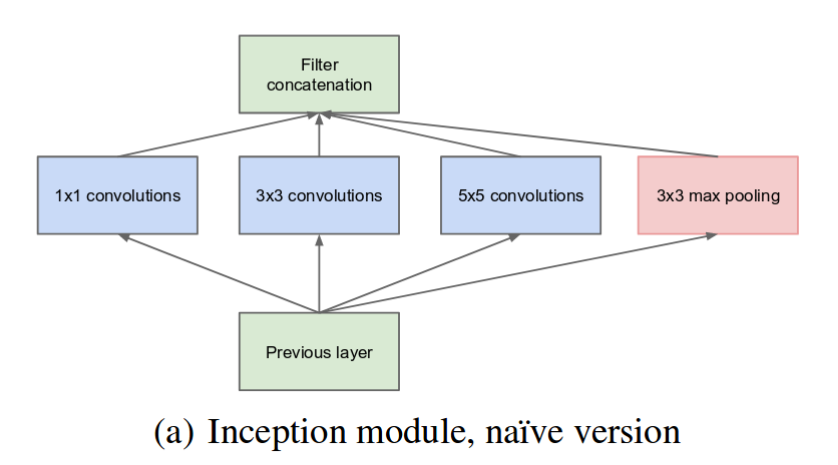
\includegraphics[width=0.95\textwidth]{img/naive-inception.png}
    \caption{The ``Naive'' inception module, image authors are Szegedy et. al.~\cite{szegedy2015Inception}.}
    \label{fig:naive-inception}
\end{figure*}

% \begin{figure*}[!ht]
%     \centering
%     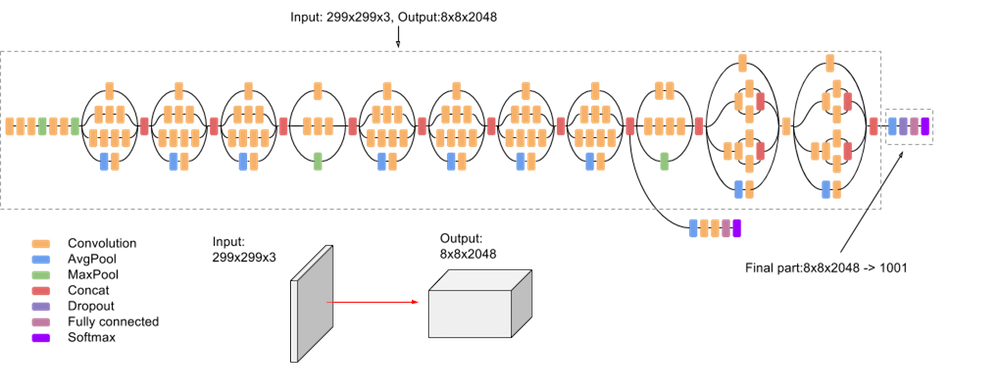
\includegraphics[width=0.95\textwidth]{img/inceptionv3.png}
%     \caption{Inception V3 Architecture\footnote{\url{https://cloud.google.com/tpu/docs/inception-v3-advanced}}.}
%     \label{fig:naive-inception}
% \end{figure*}

In order to reduce computational costs further, the authors added 1$\times$1 convolutions after the max pooling step and before the 3$\times$3 and 5$\times$5 convolutions. By doing this the authors reduce the amount of processing done by reducing the quantity of input channels before the convolutions. This improvement was named ``The inception module with dimension reduction'' and it is represented in Figure \ref{fig:red-dim-inception}.  

\begin{figure*}[!ht]
    \centering
    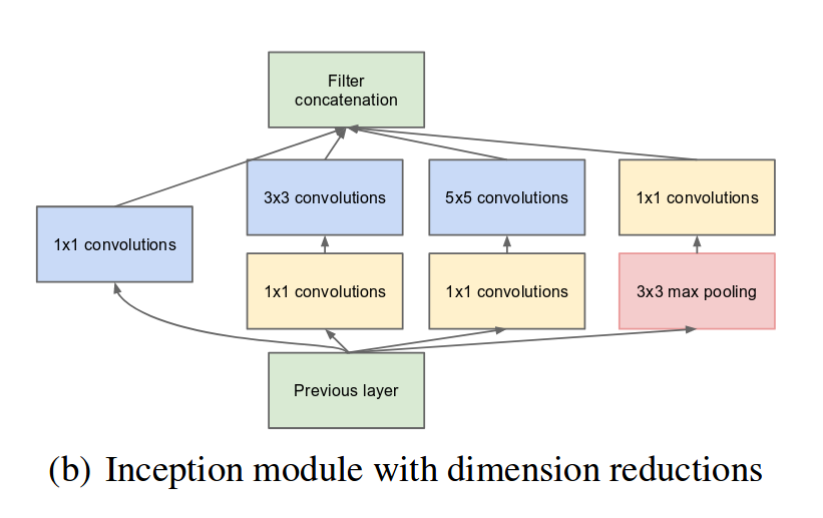
\includegraphics[width=0.95\textwidth]{img/inception-module.png}
    \caption{The inception module with dimensional reduction, image authors are Szegedy et. al.~\cite{szegedy2015Inception}.}
    \label{fig:red-dim-inception}
\end{figure*}

By stacking 9 inception modules with dimension reduction and using 2 intermediate classifiers, essentially computing prediction values and using these values to compute auxiliary losses, which are then used to compose the final loss in the training process in order to avoid the vanishing gradient problem.

As shown in Figure \ref{fig:inception-architecture} It is still deeper (it has 22 convolutional layers) than the deepest VGG configuration (with 19 convolutional layers).

\begin{figure*}[!ht]
    \centering
    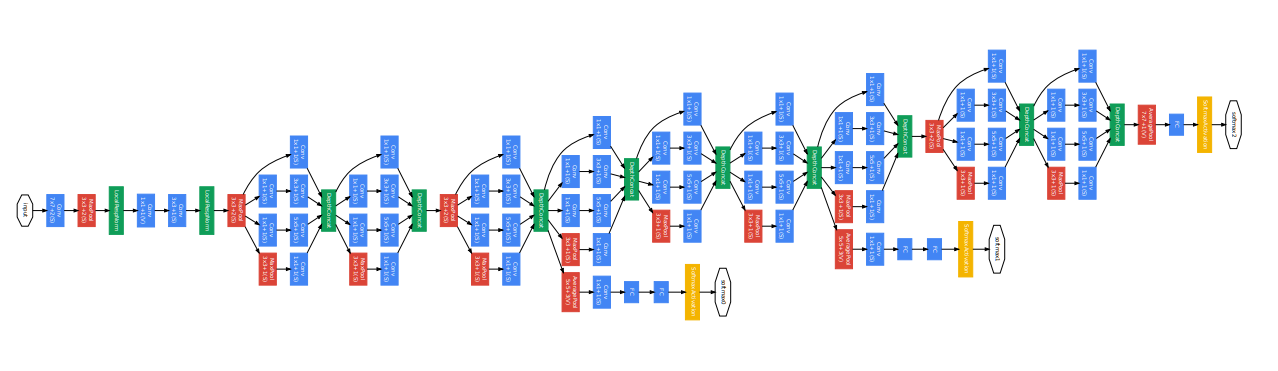
\includegraphics[width=0.95\textwidth]{img/inception-architecture.png}
    \caption{The complete inception convolutional neural network, image authors are Szegedy et. al.~\cite{szegedy2015Inception}.}
    \label{fig:inception-architecture}
\end{figure*}

InceptionV2 and InceptionV3 networks~\cite{szegedy2016rethinking}
For the inceptionV2 computational efficiency was improved by factorizing the convolutions, convolutions with 5$\times$5 size kernels were factorized into two 3$\times$3 sequential convolutions, this improves computability (because 3$\times$3 convolutions use 2.78 times less operations than 5$\times$5) while actually improving performance. They also factorized the 3$\times$3 convolutions into one 1$\times$3 and 1$\times$3 convolutions. These factorized convolutions are performed on the same input to avoid excessive dimension reduction (information loss).

The InceptionV3 CNN used all the upgrades of the InceptionV2, and improved performance further by incorporating the RMSProp Optimizer \cite{tieleman2017rmsprop}, factorized 7$\times$7 convolutions ( 1$\times$7 convolutions followed
by 7$\times$1 convolutions.), batch normalization in the Auxillary Classifiers, and Label Smoothing (It is a modification in the loss function that prevents the network having high confidence in a class) for preventing overfitting.


% RMSProp Optimizer.
% Factorized 7x7 convolutions.
% BatchNorm in the Auxillary Classifiers.
% Label Smoothing (A type of regularizing component added to the loss formula that prevents the network from becoming too confident about a class. Prevents over fitting).

The Inception CNNs continued to improve further with InceptionV4 and Inception-ResNet ~\cite{szegedy2017inceptionv4}, but we will not detail them here for they are not used in the scope of this work.


\newpage
\section{Feature Fusion}
\label{sec:feature_fusion}

Since we are using information from two different domains, image and audio, it is also important to think how one can fuse information from both these domains without . 
Which method is best to fuse the information from these different domains.

Snoek et al. \cite{snoek2005featurefusion} presents two main strategies for information fusion in semantic video analysis: 
\begin{itemize}
    \item \emph{Early fusion} methods (Figure \ref{fig:early-fusion}), which works directly with the extracted features.
    \item \emph{Late fusion} methods (Figure \ref{fig:late-fusion}), which operates on classification outputs from specialized models.
\end{itemize}

\begin{figure*}[!ht]
    \centering
    \begin{subfigure}[b]{0.55\textwidth}
        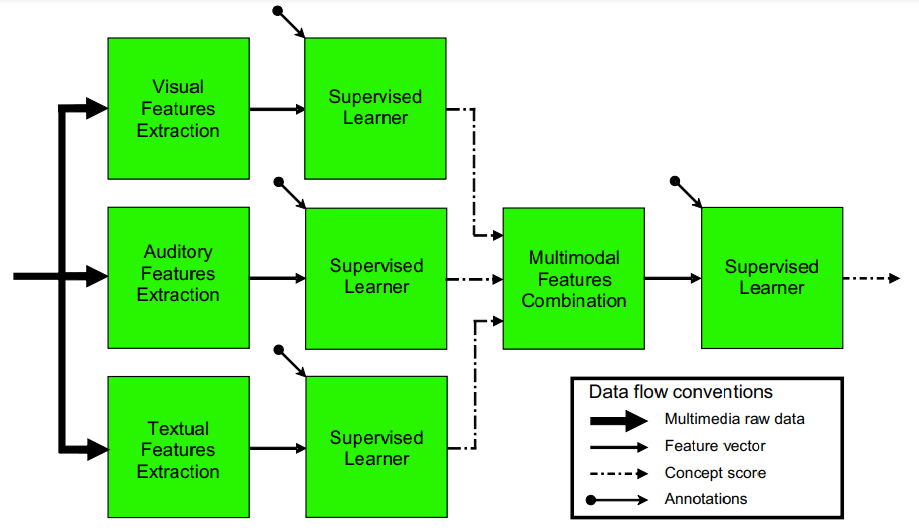
\includegraphics[width=0.94\textwidth]{img/late-fusion.png}
        \caption{The late fusion approach, in it there is a machine learning model for each unimodal feature and a final model to fuse the outputs of each unimodal model.}
        \label{fig:early-fusion}
    \end{subfigure}
    \begin{subfigure}[b]{0.44\textwidth}
        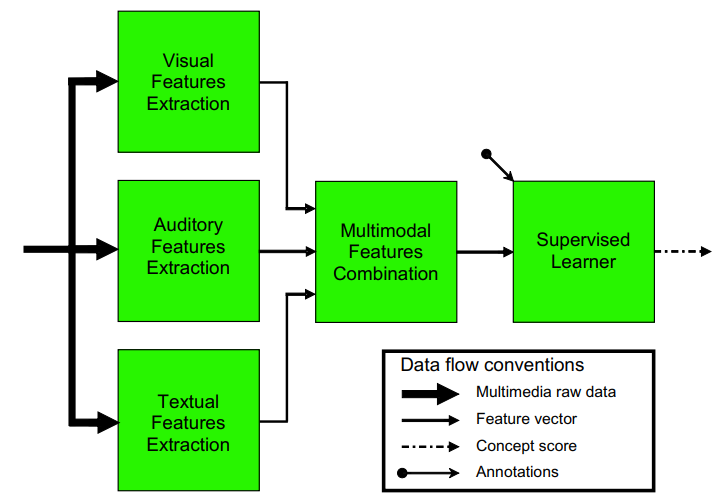
\includegraphics[width=0.94\textwidth]{img/early-fusion.png}
        \caption{The early fusion approach, it uses a single multimodal machine learning model to both aggregate and classify all features.}
        \label{fig:late-fusion}
    \end{subfigure}
    \caption{The late and early fusion methods for feature fusion. Image authors are Snoek et. al.~\cite{snoek2005featurefusion}.}
\end{figure*}


% late fusion comes at cost of training time
In the work by Snoek et. al.\cite{snoek2005featurefusion}, the Late fusion approach tends to give better performance on most semantic concepts (multilabel video classification) at the cost of increased computability costs. However, the authors also conclude that the late and early fusion approaches should be compared are per concept (in a multilabel situation).%, which one can generalize to per task in binary tasks.